\section{Marco Teórico}

\subsubsection*{Panel fotovoltaico}
Su funcionamiento se basa en el efecto fotoeléctrico, este fenómeno dice que al incidir fotones en un material conductor o semiconductor, se desprenden electrones de este mismo, esto ocurre debido  a que la energía del fotón incidente es absorbida por un electrón en el metal, generando un desprendimiento de algunos electrones.[1]\\

En este contexto, se usa un material semiconductor que al llegar al equilibrio de potencial,en las junturas p-n se genera una zona marcada de diferencia potencial (flujo de campo eléctrico $E$ marcado)

\begin{figure}[h]
    \centering
    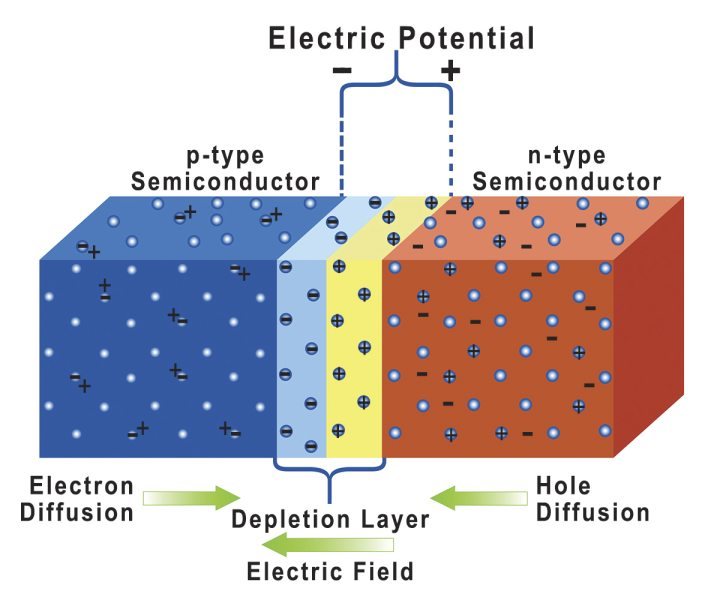
\includegraphics[width=0.25\linewidth]{imageneees/rSjj0.jpg}
    \caption{Diagrama juntura p-n, se puede apreciar la diferencia de potencial generando un campo eléctrico}
    \label{fig:placeholder}
\end{figure}\\

Este 'equilibrio' generador en la juntura p-n se romperá en el caso de que se arranque un electrón del material, generando un flujo de corriente por esto mismo, aprovechando este comportamiento básico es donde se crea el panel fotovoltaico para aprovechar este fenómeno y generar electricidad a partir de energía solar.\\

El panel fotovoltaico esta hecho de células fotoeléctricas, estas células están hechos de un material semiconductor, las cuáles generan electricidad ($1$ a $2$ $[W]$ por celda)[2]  se pueden conectar varias células para formar paneles fotovoltaicos más grandes. Se puede modelar el comportamiento de un panel fotovoltaico y sus pérdidas mediante el siguiente circuito equivalente:\\
\begin{figure}[H]
    \centering
    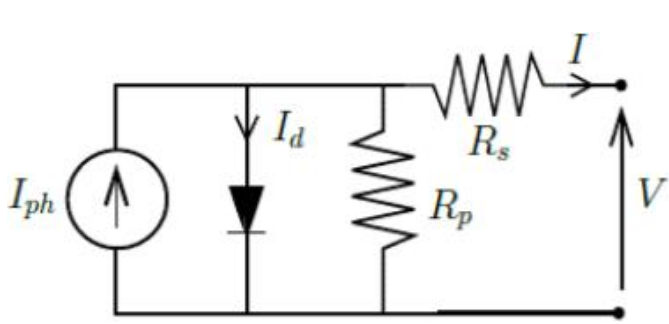
\includegraphics[width=0.5\linewidth]{imageneees/imagen.png}
    \caption{Circuito equivalente simplificado celda fotovoltaica}
    \label{fig:placeholder}
\end{figure}
Donde \begin{itemize}
    \item El diodo aparece gracias a que las células fotoeléctricas están hechas de un material semiconductor con juntura p-n, el cuál se puede modelar como un diodo
    \item $R_{s}:$ pérdidas por conducción gracias a elementos internos del panel como la interconexión, cableado , resistencia del material, entre otros.
    \item $R_{p}:$ defectos en la fabricación en la juntura semiconductora
\end{itemize}

\subsection{Curva I-V}
Para construir esta curva necesitamos la corriente de cortocircuito $I_{cc}$y la tensión en circuito abierto $V_{ca}$, para obtenerlas hay que hacer las pruebas correspondientes al panel y obtener estos parámetros antes mencionados. 

\subsubsection{Prueba cortocircuito y circuito abierto}
Para la prueba de cortocircuito hay que hacerle un cortocircuito a los terminales del panel fotoeléctrico, mientras que para obtener el voltaje en circuito abierto, hay que calcular este parámetro sin ninguna carga conectada al panel solar.\\

Con esta información se puede construir la curva I-V:
\begin{figure}[H]
    \centering
    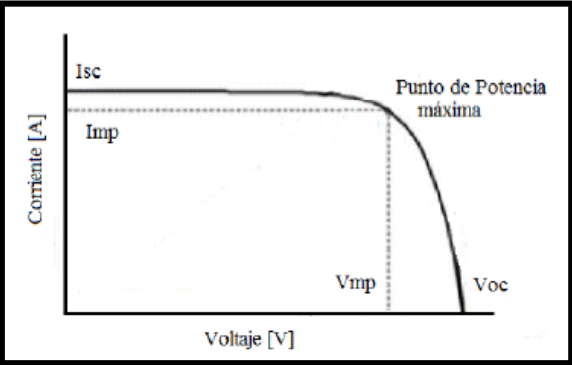
\includegraphics[width=0.5\linewidth]{imageneees/132412.png}
    \caption{Curva I-V panel fotovoltaico}
    \label{fig:placeholder}
\end{figure}[H]
Donde \begin{itemize}
    \item $I_{SC}:\text{corriente de cortocircuito}$
    \item $V_{OC}:\text{tensión en circuito abierto}$
    \item MPP: Punto de potencia máxima
\end{itemize}\\

Dependiendo de la irradiancia y la temperatura esta curva se va desplazando dependiendo de que parámetro varía.


\textbf{Irradiancia:} radiación incidente por unidad de superficie. Indica la intensidad de la radiación solar, se mide en $\left[\frac{W}{m^2}\right]$ [3]\\
Mientras mayor irradiancia, mayor el módulo de la corriente.
\begin{figure}[H]
    \centering
    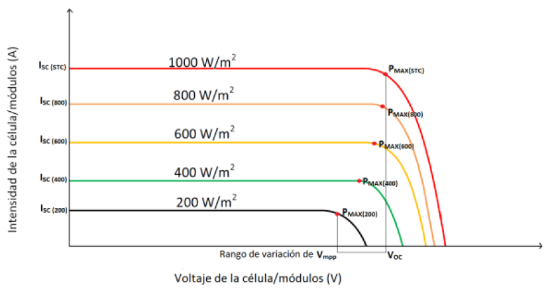
\includegraphics[width=0.5\linewidth]{imageneees/41241421en.png}
    \caption{Gráfico I-V, donde las distintas curvas representan distintos niveles de irradiancia}
    \label{fig:placeholder}
\end{figure}
\\
\textbf{Temperatura:} La temperatura ambiente a la que esta el panel fotovoltaico desplaza mi curva $V-I$ en el eje x (tensión), donde a mayor temperatura, se alcanzará más rápido el punto de potencia máxima en comparación con temperatura ambiente baja, es decir, en temperaturas altas, cae la tensión y en temperaturas bajas, sube la tensión.

\begin{figure}[H]
    \centering
    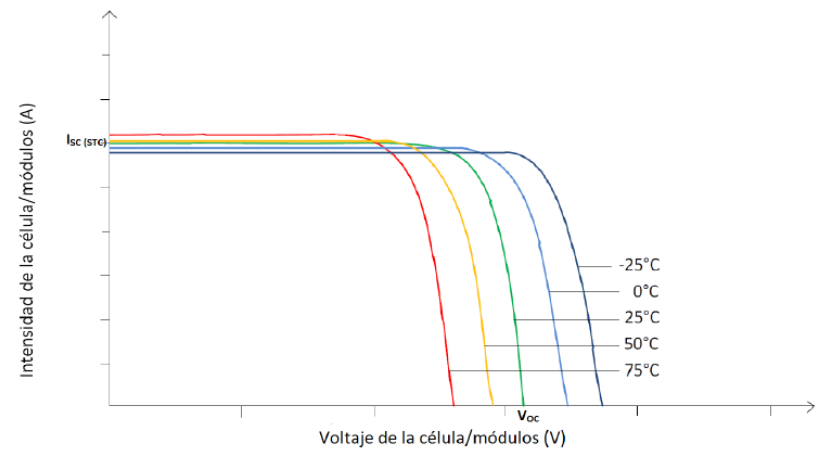
\includegraphics[width=0.5\linewidth]{imageneees/12131.png}
    \caption{Gráfico I-V, donde las distintas curvas representan distintos niveles de temperatura}
    \label{fig:placeholder}
\end{figure}

\subsection{Efecto sombra}
Cuando las células fotovoltaicas son sombreadas, pasan a tener un comportamiento resistivo, produciendo una caída de tensión e invirtiendo al polaridad [4], como tiene este comportamiento se disipa calor debido al efecto Joule o llamado "Hot spot" en este caso. Este calentamiento ádemas de afectar la cantidad de energía generada por el panel, puede dañar o destruir por completo la(s) celula(s), es por eso que en la construcción de paneles fotovoltaicos es muy importante tener medidas para impedir/ aislar el efecto sombra, generalmente se usa un diodo byPass para \textbf{aislar} las células que estan sufriendo el efecto sombra.

\subsubsection{Diodo byPass para tratar el efecto sombra}\\

En la práctica se conectan más de un diodo byPass en paralelo en mis paneles, esto con el fin de evitar el efecto sombra en toda el área del panel, el diodo esta conectado en paralelo con polaridad opuesta, aprovechandose de que cuando una célula es afectada por el efecto sombra, esta cambia de polaridad, "activandose" así el diodo, el cuál desvía la corriente que iba a pasar por la(s) célula(s) afectadas por el efecto sombra anteriormente, pasando por el diodo Bypass, asegurando que las celdas no sombradas puedan seguir generando.
\begin{figure}[h]
    \centering
    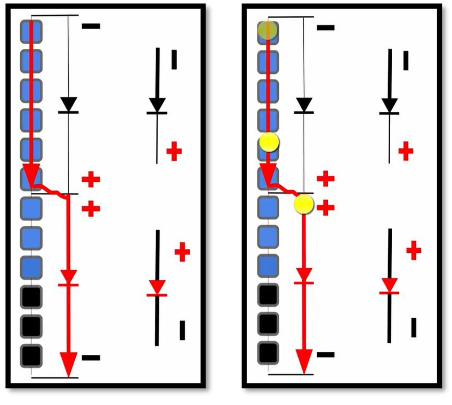
\includegraphics[width=0.35\linewidth]{imageneees/55513251.png}
    \caption{Efecto diodo Bypass en un panel fotovoltaico donde una parte de él esta bajo el  efecto sombra}
    \label{fig:placeholder}
\end{figure}



\newpage
\subsection*{Energía eólica}
\subsubsection*{Origen de las corrientes de aire} Las corrientes de aire y sus distintas magnitudes y direcciones dependiendo de la ubicación geográfica depende de 3 factores principales : \begin{enumerate}
    \item \textbf{Radiación solar y rotación de la tierra:} Se produce un calentamiento no uniforme de la superficie terrestre, esto principalmente debido a la trayectoria elíptica que sigue la tierra y que la tierra rota sobre sí misma. [5]
    \item \textbf{Otros factores atmosféricos:} Si bien las condiciones atmosféricas cómo la presencia de nubes afectan en parte la cantidad efectiva de radiación que llega a la superficie terrestre, el principal parámetro que afecta la cantidad efectiva de radiación es el \textbf{ángulo cenital}, mientras más pequeño este ángulo, más 'corto' es el trayecto que toma la luz, por lo tanto, menor atenuación de la radiación habrá.\\

\end{enumerate}

La presencia de estos 3 factores producen que la velocidad de el aire no sea un valor constante, sino que tenga una variabilidad asociada la cuál depende de las condiciones climáticas, superficiales del terreno, la hora actual, estaciones del año,variabilidad intrínseca de las condiciones eólicas, entre otros.\\

Es importante mencionar que el potencial  del viento (movimiento de las masas de aire),va desde áreas de mayor a menor presión.

\begin{figure}
    \centering
    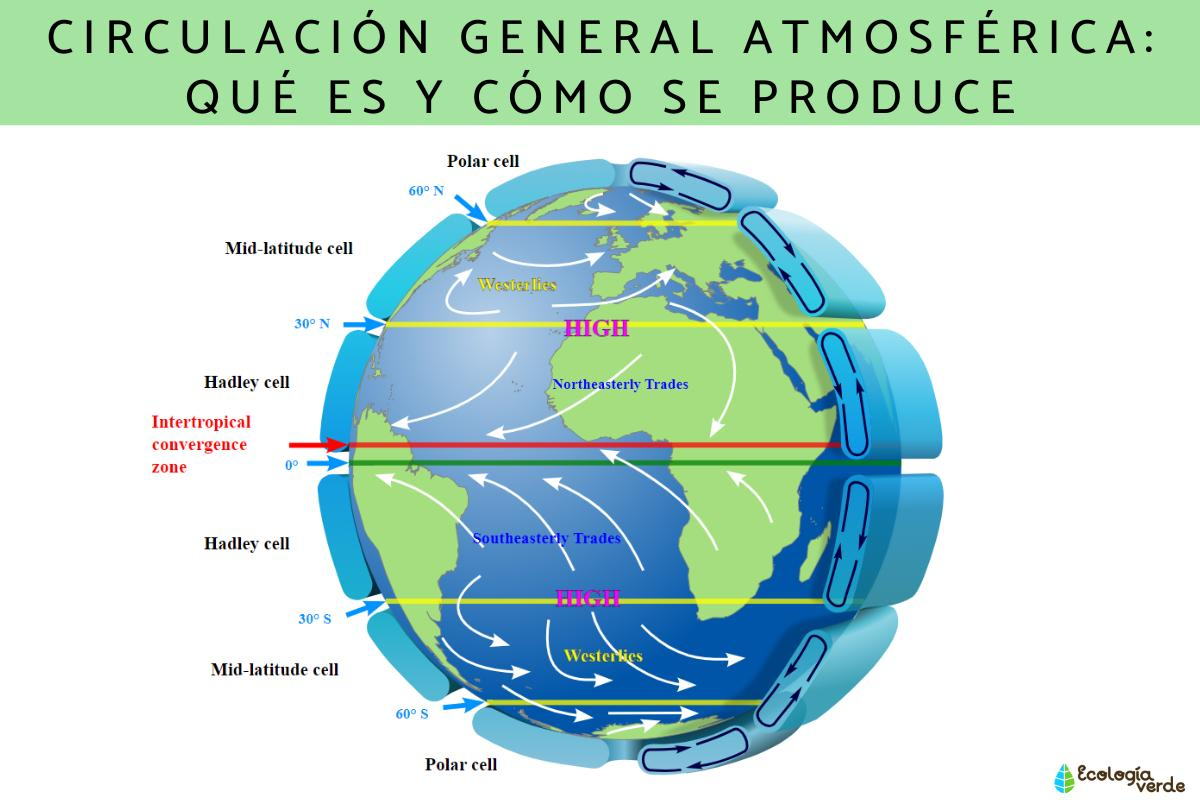
\includegraphics[width=0.5\linewidth]{imageneees/circulacion_general_atmosferica_que_es_y_como_se_produce_5126_orig.jpg}
    \caption{Mapeo simplificado de las direcciones del aire dependiendo de la latitud}
    \label{fig:placeholder}
\end{figure}
\newpage
\subsection*{Turbina eólica}
El funcionamiento principal de la turbina eólica es convertir potencia mecánica $P_{m}$ en electricidad.\\

La máxima potencia que una turbina eólica puede extraer del viento viene dada por la siguiente ecuación:$$P_{máx}^{aire}=\frac{1}{2}\cdot \rho \cdot A \cdot v^3$$ Donde el área A es un área virtual que definimos cómo el área donde el viento atraviesa perpendicularmente esta misma.
\begin{figure}
    \centering
    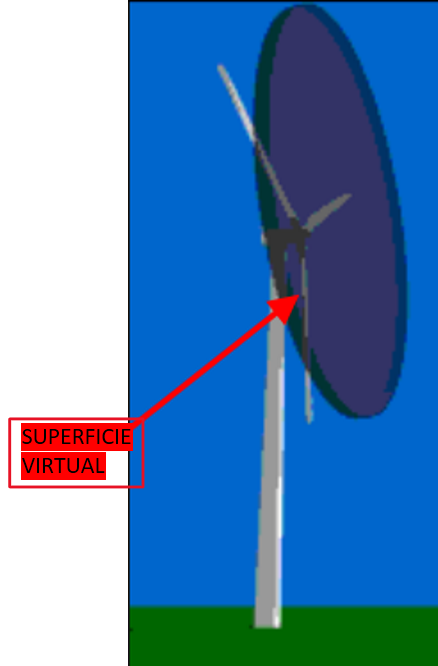
\includegraphics[width=0.20\linewidth]{imageneees/555.png}
    \caption{Superficie virtual arbitraria en una turbina eólica}
    \label{fig:placeholder}
\end{figure}
\\

Según la ley de Bentz, se puede convertir solo el $59\%$ de la potencia que posee el viento, esto es un límite teórico por lo que en la práctica, el porcentaje de potencia máxima obtenida es mucho menor, pues no tenemos ni equipos con eficiencia $\infty$ y las condiciones no son ideales, sin embargo, las nuevas tecnologías y técnicas se intentan acercar lo más posible a este valor.

\subsubsection{Curva P-$\omega$}
Donde $\omega$ es la velocidad del viento $[\frac{m}{s}]$ y P es la potencia generada por la turbina eólica.
\begin{figure}
    \centering
    \includegraphics[width=0.4\linewidth]{1231234.png}
    \caption{Curva P-$\omega$ turbina eólica}
    \label{fig:hola}
\end{figure}
Donde se puede observar 3 puntos importantes:\\

\begin{enumerate}
    \item \textbf{Cut-in-speed:} es el punto indicado en la figura \ref{fig:hola}, esta es la velocidad del viento mínima requerida para que funciona la turbina eólica, físicamente es la velocidad requerida para que se supere la inercia de la turbina y empiece a girar.
    \item \textbf{Cut-out-speed:} es el punto indicado en la figura \ref{fig:hola}, es la máxima velocidad del viento permitida, en este punto se activan las protecciones y la turbina sale de funcionamiento.
    \item \textbf{Máxima potencia generada:} En la misma figura, en el intervalo de $w'$ donde la potencia $P_{w'}$ es constante, es la potencia máxima que puede entregar la turbina.
\end{enumerate}
\begin{figure}
    \centering
    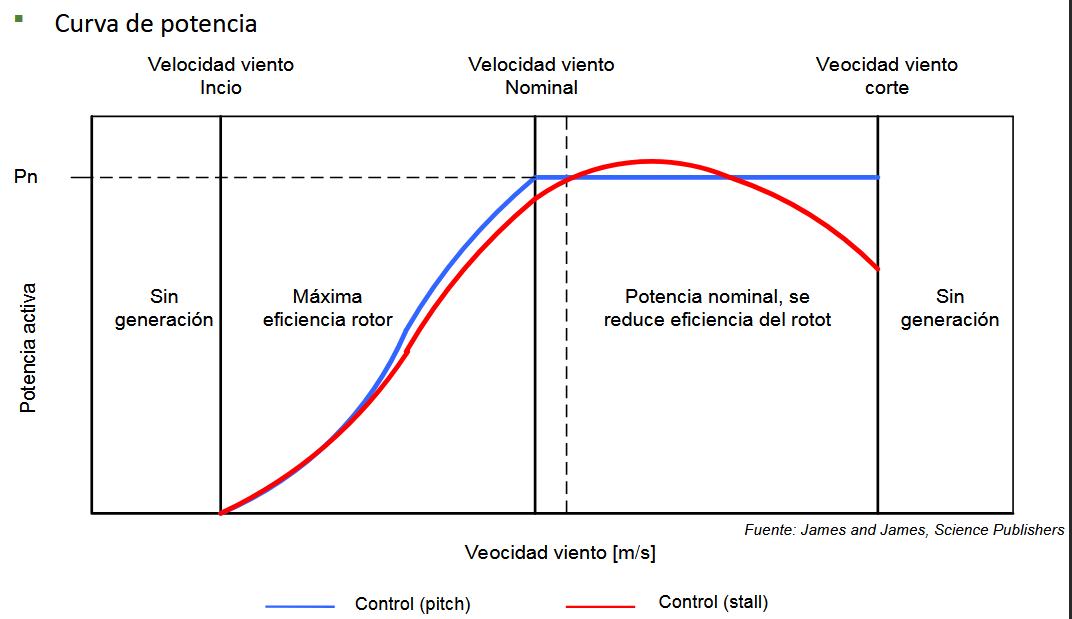
\includegraphics[width=0.85\linewidth]{imageneees/13255125.png}
    \caption{Explicación curva P-$\omega$ por tramos}
    \label{fig:bla}
\end{figure}
Podemos concluir del gráfico \ref{fig:bla} que al alcanzar la velocidad nominal del viento (parámetro que depende del tipo de turbina) , la la potencia que entrega la turbina eólica es máxima 'Potencia nominal'.
